% Paper 12 frozen figure inclusion, caption, and label contract.
% Exactly three proof-navigation figures. No result/runtime-derived plots.

\begin{figure*}[t]
  \centering
  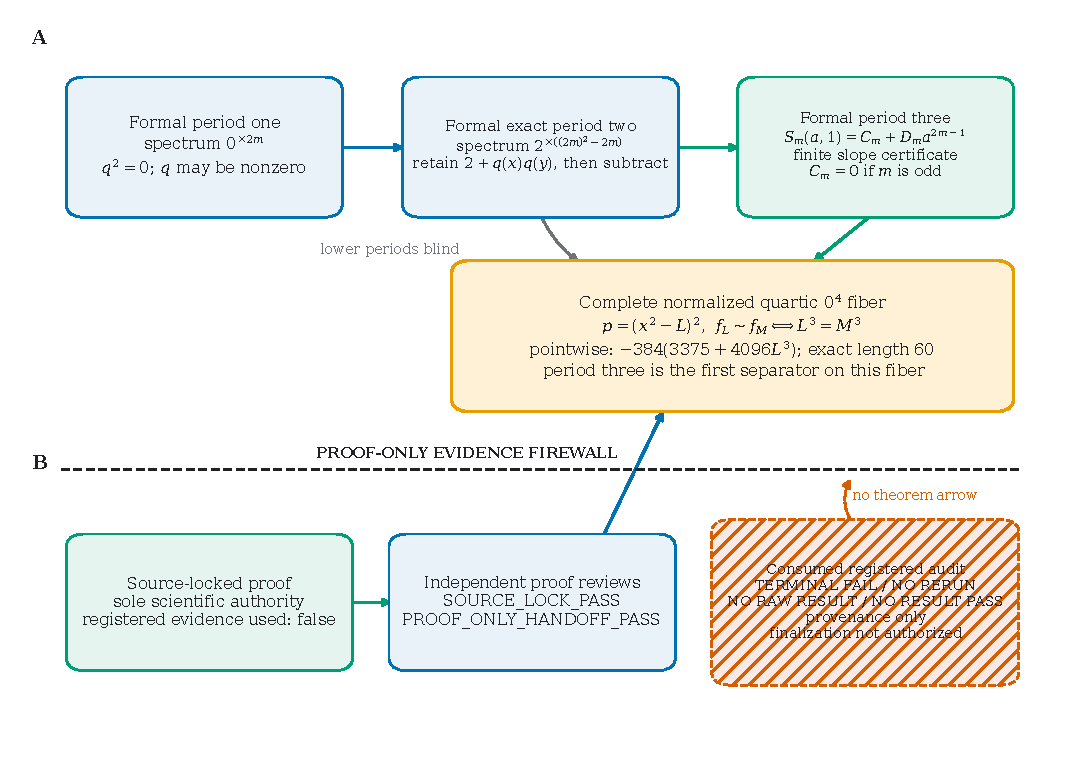
\includegraphics[width=\textwidth]{figures/fig1_theorem_architecture.pdf}
  \caption{Theorem architecture and evidence boundary. The formal
  period-one and exact-period-two multiplication spectra are constant on the
  normalized family, with nilpotent corrections retained before passing to
  spectra. The period-three cyclic complete intersection yields the two-term
  moment law and, on the complete normalized quartic fiber with formal
  fixed-point trace multiset $0^4$, the exact pointwise moment
  $-384(3375+4096L^3)$, formal exact-period-three length $60$, and minimal
  separation by $L^3$. Every arrow into a theorem box originates in the
  source-locked proof and independent proof reviews. The consumed registered
  audit contributes only the dashed provenance branch: it terminally failed,
  supplies no scientific evidence, and authorizes neither a result claim nor
  finalization.}
  \label{fig:theorem-architecture}
\end{figure*}

\begin{figure*}[t]
  \centering
  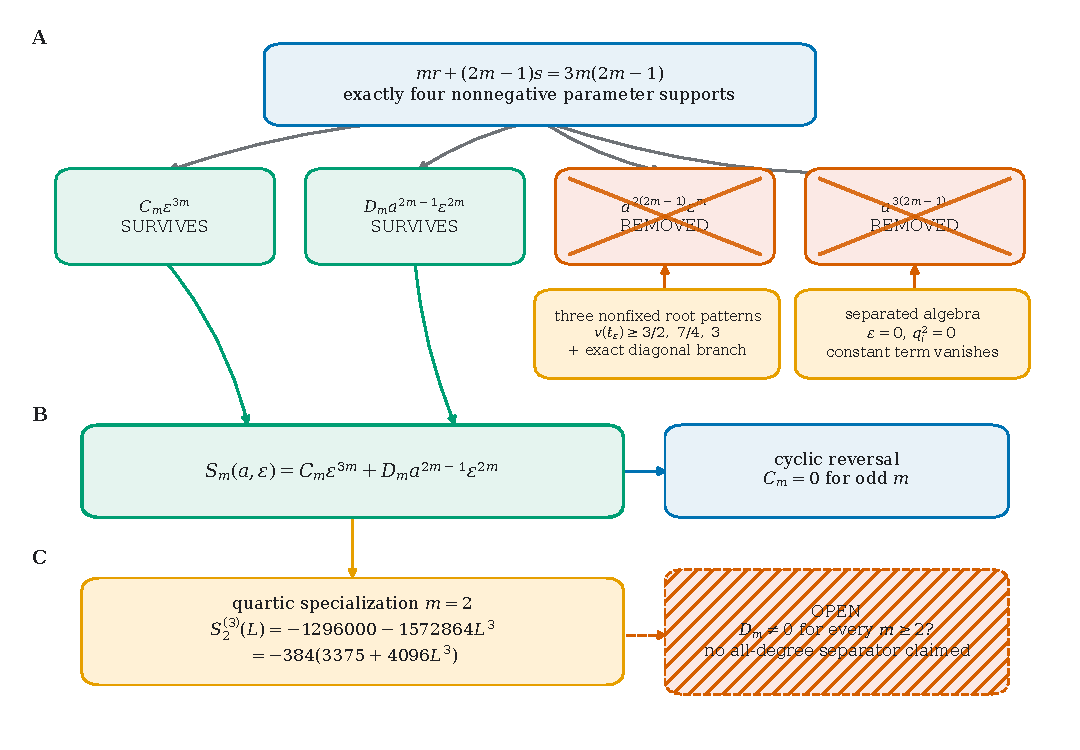
\includegraphics[width=\textwidth]{figures/fig2_weighted_two_term_law.pdf}
  \caption{Weighted support and the two-term law. Weighted homogeneity
  permits exactly four parameter monomials in $S_m(a,\varepsilon)$. The
  separated algebra at $\varepsilon=0$ removes $a^{3(2m-1)}$, and the three
  nonfixed degeneration patterns together with the exact diagonal branch
  remove $a^{2(2m-1)}\varepsilon^m$. The surviving terms are
  $C_m\varepsilon^{3m}$ and $D_ma^{2m-1}\varepsilon^{2m}$; cyclic reversal
  additionally gives $C_m=0$ for odd $m$. For $m=2$, source-level
  coefficient derivations give
  $S_2^{(3)}(L)=-1296000-1572864L^3$. The diagram makes no universal
  separation claim: $D_m\neq0$ for every $m\geq2$ remains open.}
  \label{fig:weighted-two-term-law}
\end{figure*}

\begin{figure*}[t]
  \centering
  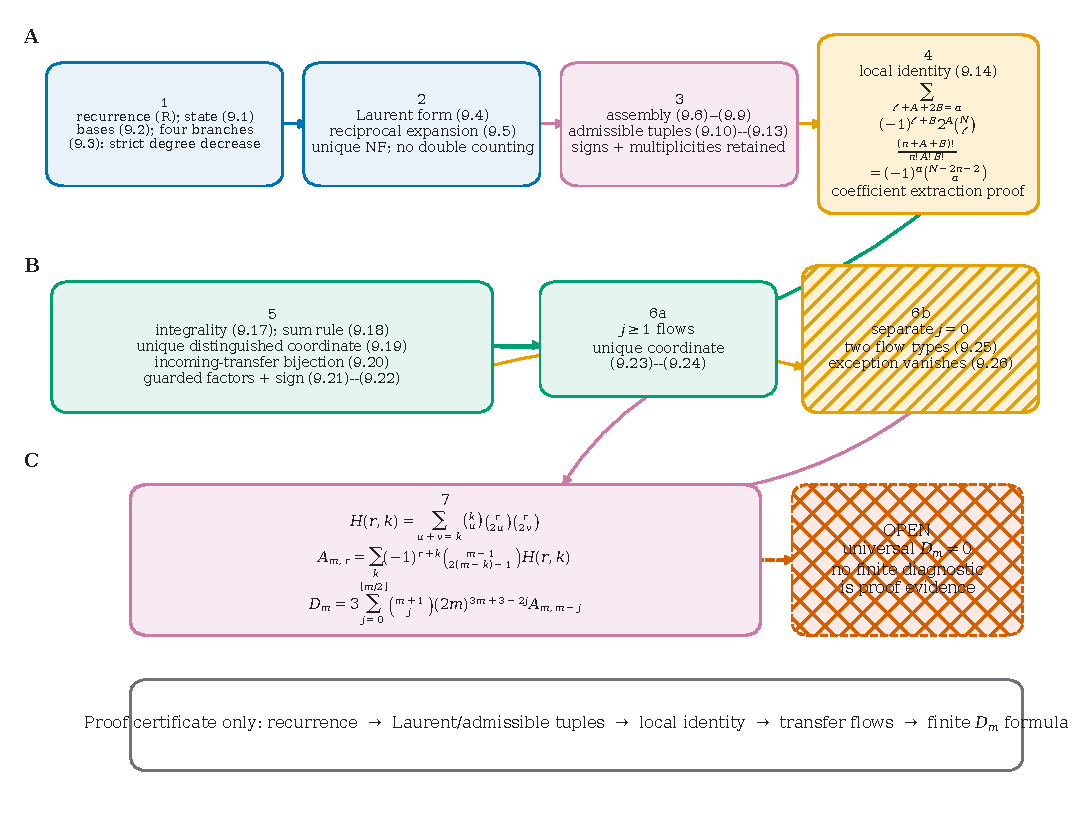
\includegraphics[width=\textwidth]{figures/fig3_step9_certificate_pipeline.pdf}
  \caption{Transparent coefficient-certificate pipeline. The four-branch
  recurrence and base cases terminate by strict total-degree decrease; the
  Laurent coefficient makes the reduction order independent and groups
  branch interleavings without double counting. Admissible tuples retain
  every sign, multiplicity, Laurent exponent, and parameter degree. The local
  identity (9.14), proved by one-variable coefficient extraction, collapses
  each signed fiber. For $j\geq1$, a unique distinguished coordinate and an
  incoming-transfer bijection give the guarded $H/A$ factors; $j=0$ is
  handled by a separate exhaustive flow classification, including the
  vanishing exceptional pattern. Assembly yields the finite formula for
  $D_m$. Universal $D_m\neq0$ is explicitly open, and no runtime or finite
  diagnostic is part of this proof.}
  \label{fig:step9-certificate-pipeline}
\end{figure*}
